\documentclass{beamer}
\usepackage[utf8]{inputenc}
\usepackage{graphicx, epsfig}
\usepackage{amsmath,mathrsfs,amsfonts,amssymb}
%\usepackage{subfig}
\usepackage{floatflt}
\usepackage{epic,ecltree}
\usepackage{mathtext}
\usepackage{fancybox}
\usepackage{fancyhdr}
\usepackage{multirow}
\usepackage{enumerate}
\usepackage{epstopdf}
\usepackage{multicol}
\usepackage{algorithm}
\usepackage[noend]{algorithmic}
\def\algorithmicrequire{\textbf{Input:}}
\def\algorithmicensure{\textbf{Output:}}
\usetheme{default}%{Singapore}%{Warsaw}%{Warsaw}%{Darmstadt}
\usecolortheme{default}
\setbeamertemplate{footline}[page number]{}
\setbeamerfont{title}{size=\Huge}

\newcommand{\bt}{\mathbf{t}} 
\newcommand{\bu}{\mathbf{u}} 
\newcommand{\bv}{\mathbf{v}} 
\newcommand{\bw}{\mathbf{w}} 
\newcommand{\bx}{\mathbf{x}} 
\newcommand{\bz}{\mathbf{z}} 
\newcommand{\by}{\mathbf{y}} 

\newcommand{\bI}{\mathbf{I}} 
\newcommand{\bT}{\mathbf{T}} 
\newcommand{\bX}{\mathbf{X}} 
\newcommand{\bZ}{\mathbf{Z}} 

\newcommand{\bepsilon}{\boldsymbol{\epsilon}}
\newcommand{\bmu}{\boldsymbol{\mu}}
\newcommand{\blambda}{\boldsymbol{\lambda}}
\newcommand{\bsigma}{\boldsymbol{\sigma}}
\newcommand{\bSigma}{\boldsymbol{\Sigma}}

\newcommand{\btheta}{\boldsymbol{\theta}} 
\newcommand{\bphi}{\boldsymbol{\phi}} 

\DeclareMathOperator*{\argmin}{arg\,min}
\DeclareMathOperator*{\argmax}{arg\,max}

%\definecolor{beamer@blendedblue}{RGB}{15,120,80}
%----------------------------------------------------------------------------------------------------------
\title[\hbox to 56mm{Deep Generative Models  \hfill\insertframenumber\,/\,\inserttotalframenumber}]
{Deep Generative Models \\ Lecture 7}
\author[Roman Isachenko]{\\Roman Isachenko}
\institute[MIPT]{Moscow Institute of Physics and Technology \\
}
\date{2020}
%--------------------------------------------------------------------------------
\begin{document}
%--------------------------------------------------------------------------------
\begin{frame}
%\thispagestyle{empty}
\titlepage
\end{frame}
%=======
\begin{frame}{VAE limitations}
	\begin{itemize}
		\item Poor variational posterior distribution (encoder)
		\[
		q(\bz | \bx, \bphi) = \mathcal{N}(\bz| \bmu_{\bphi}(\bx), \bsigma^2_{\bphi}(\bx)).
		\]
		\item Poor prior distribution
		\[
		p(\bz) = \mathcal{N}(0, \mathbf{I}).
		\]
		\item Poor probabilistic model (decoder)
		\[
		p(\bx | \bz, \btheta) = \mathcal{N}(\bx| \bmu_{\btheta}(\bz), \bsigma^2_{\btheta}(\bz)).
		\]
		\item Loose lower bound
		\[
		p(\bx | \btheta) - \mathcal{L}(q, \btheta) = (?).
		\]
	\end{itemize}
\end{frame}
%=======
\begin{frame}{VAE prior}
	\begin{block}{ELBO revisiting}
		\vspace{-0.3cm}
		{\footnotesize
			\[
			\mathcal{L}(q, \btheta) = \underbrace{\frac{1}{n} \sum_{i=1}^n \mathbb{E}_{q(\bz_i | \bx_i)} \log p(\bx_i | \bz_i, \btheta)}_{\text{Reconstruction loss}} - \underbrace{\left(\log n - \mathbb{E}_{q(\bz)} \mathbb{H} \left[ q(i | \bz) \right] \right)\vphantom{\sum_{i=1}}}_{0 \leq \text{Mutual info} \leq \log N } - \underbrace{KL(q(\bz) || p(\bz))\vphantom{\sum_{i=1}}}_{\text{Marginal KL}}
			\]}
	\end{block}
	
	How to choose the optimal $p(\bz)$?
	\begin{itemize}
		\item SG: $p(\bz) = \mathcal{N}(0, I)$ $\Rightarrow$ over-regularization;
		\vspace{0.1cm}
		\item MoG: $p(\bz | \blambda) = \frac{1}{K} \sum_{k=1}^K \mathcal{N}(\bmu_k, \bsigma_k^2)$ $\Rightarrow$ (*), (**);
		\vspace{0.1cm}
		\item $p(\bz) = q(\bz) = \frac{1}{n}\sum_{i=1}^n q(\bz | \bx_i)$ $\Rightarrow$ overfitting and highly expensive.
	\end{itemize}
	\vfill
	\hrule\medskip
	{\tiny 
		(*) \href{https://arxiv.org/abs/1611.02648}{https://arxiv.org/abs/1611.02648} \\
		(**) \href{https://pdfs.semanticscholar.org/f6fe/5e8e25994c188ba6a124462e2cc55f2c5a67.pdf}{https://pdfs.semanticscholar.org/f6fe/5e8e25994c188ba6a124462e2cc55f2c5a67.pdf}}
	
\end{frame}
%=======
\begin{frame}{VampPrior, 2017}
	\begin{block}{Variational Mixture of posteriors}
		\[
		p(\bz | \blambda) = \frac{1}{K} \sum_{k=1}^K q(\bz | \bu_k),
		\]
		where $\blambda = \{\bu_1, \dots, \bu_K\}$ are trainable preudo-inputs.
	\end{block}
	\begin{itemize}
		\item Multimodal $\Rightarrow$ prevents over-regularization;.
		\item $K \ll n$ $\Rightarrow$ prevents from potential overfitting + less expensive to train.
		\item Pseudo-inputs are prior hyperparameters $\Rightarrow$ connection to the Empirical Bayes.
	\end{itemize}
	\vfill
	\hrule\medskip
	{\scriptsize \href{https://arxiv.org/pdf/1705.07120.pdf}{https://arxiv.org/pdf/1705.07120.pdf}}
\end{frame}
%=======
\begin{frame}{VampPrior, 2017}
	Do we equally need the multimodal prior? \\
	\vspace{0.2cm}
	Is it beneficial to couple the prior with the variational posterior or MoG is enough?
	\begin{minipage}[t]{0.5\columnwidth}
		\begin{figure}[h]
			\centering
			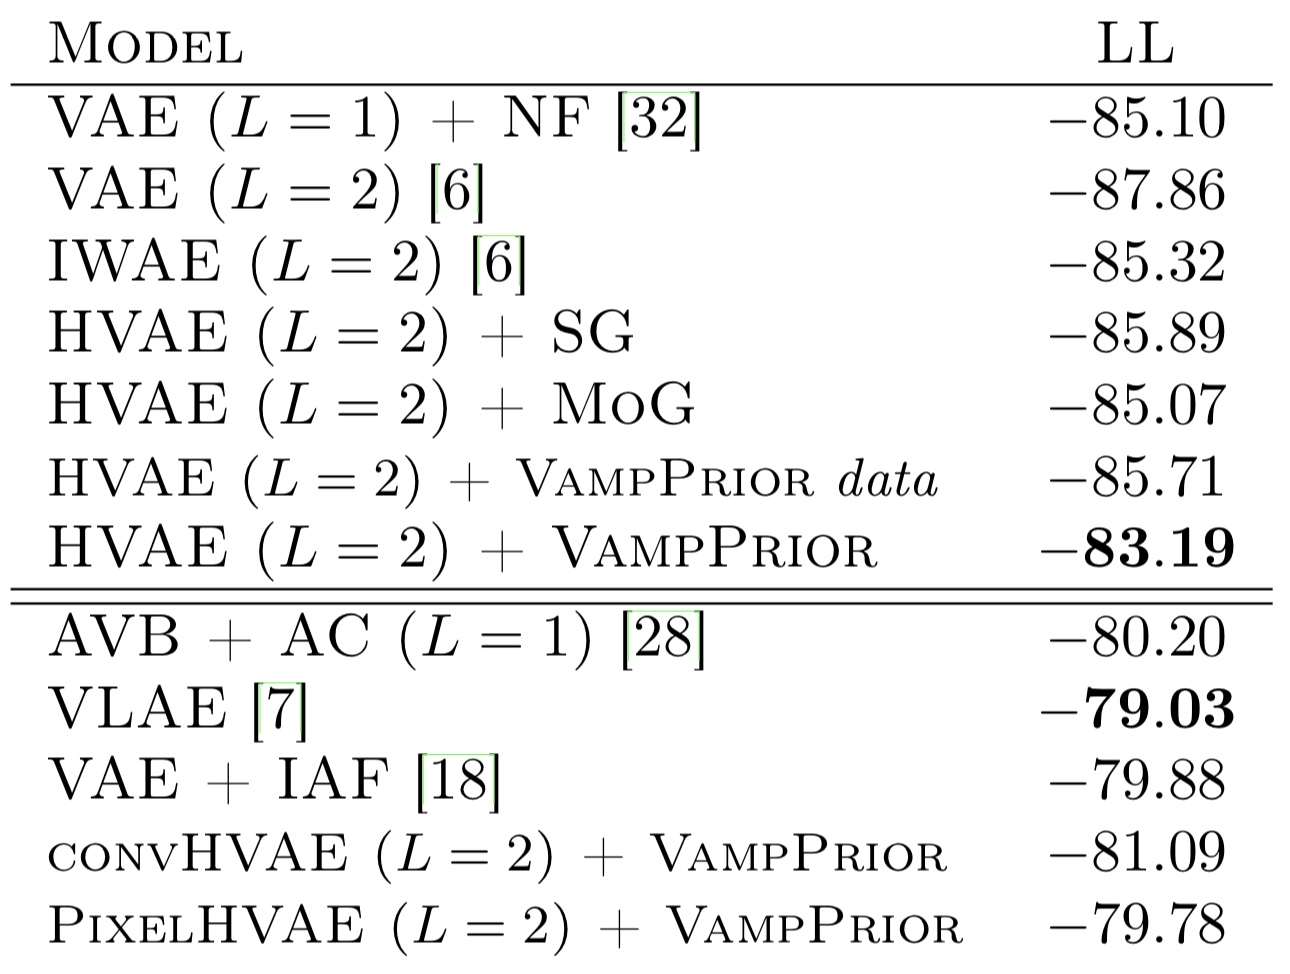
\includegraphics[width=1.\linewidth]{figs/VampPrior_1.png}
		\end{figure}
	\end{minipage}%
	\begin{minipage}[t]{0.5\columnwidth}
		\begin{figure}[h]
			\centering
			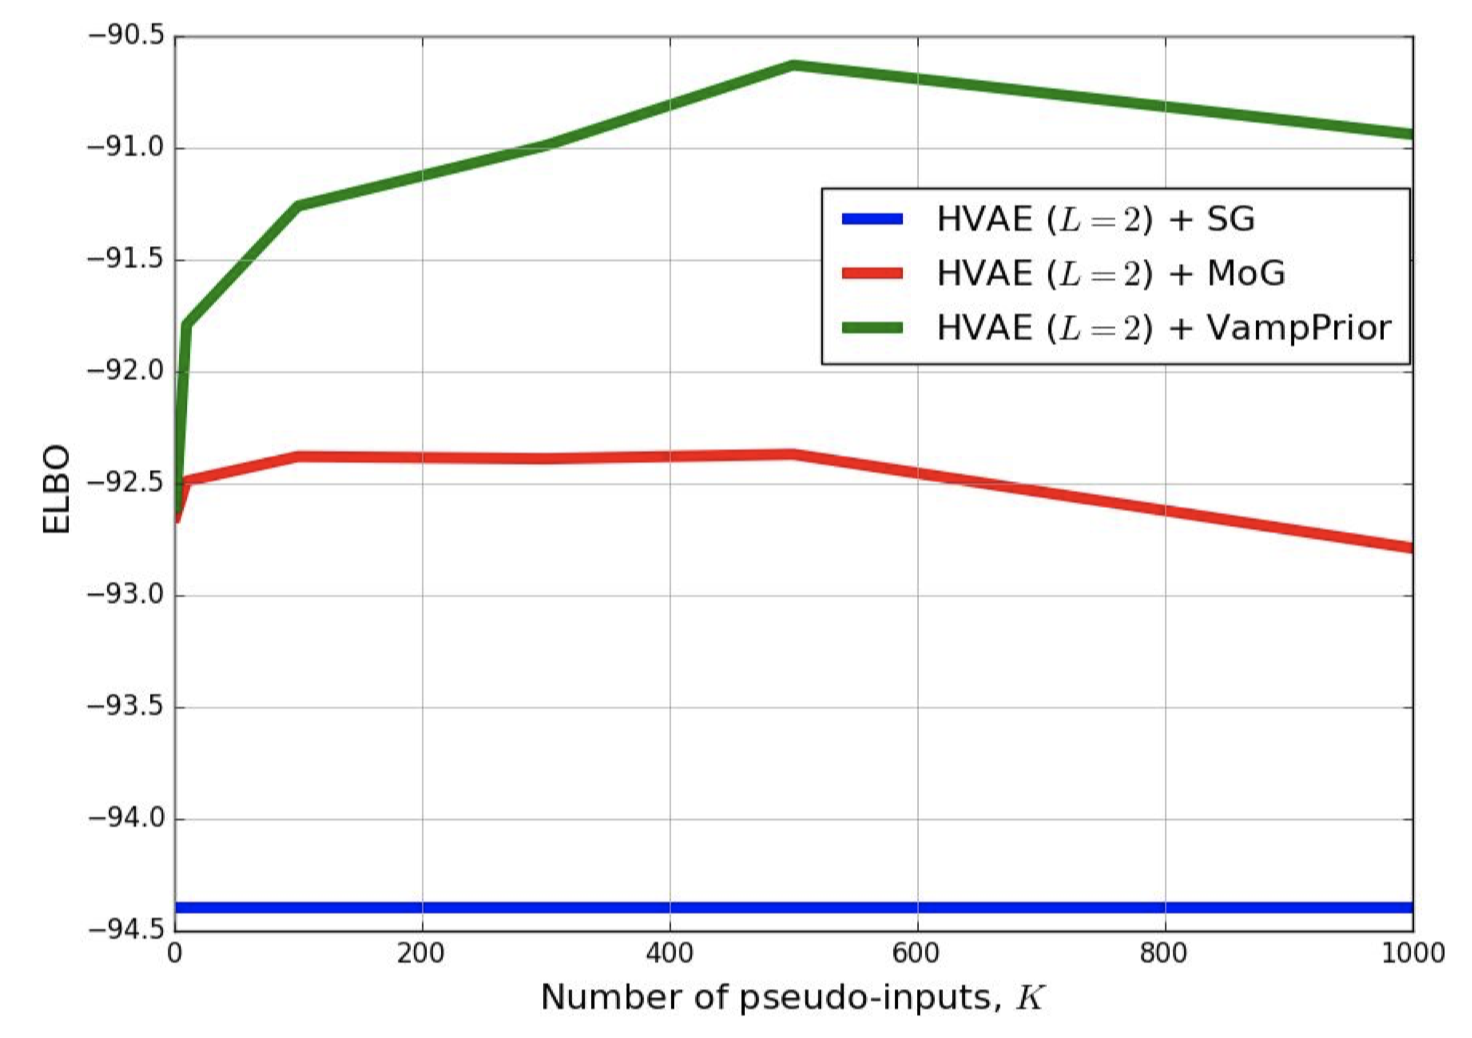
\includegraphics[width=1.\linewidth]{figs/VampPrior_2.png}
		\end{figure}
	\end{minipage}
	\vfill
	\hrule\medskip
	{\scriptsize \href{https://arxiv.org/pdf/1705.07120.pdf}{https://arxiv.org/pdf/1705.07120.pdf}}
\end{frame}
%=======
\begin{frame}{VampPrior, 2017}
	\vspace{0.1cm}
	\textbf{Top row:} images generated by PixelHVAE + VampPrior for chosen pseudo-input in the left top corner. \\
	\vspace{0.1cm}
	\textbf{Bottom row:} Images represent a subset of trained pseudo-inputs for different datasets.
	\begin{figure}[h]
		\centering
		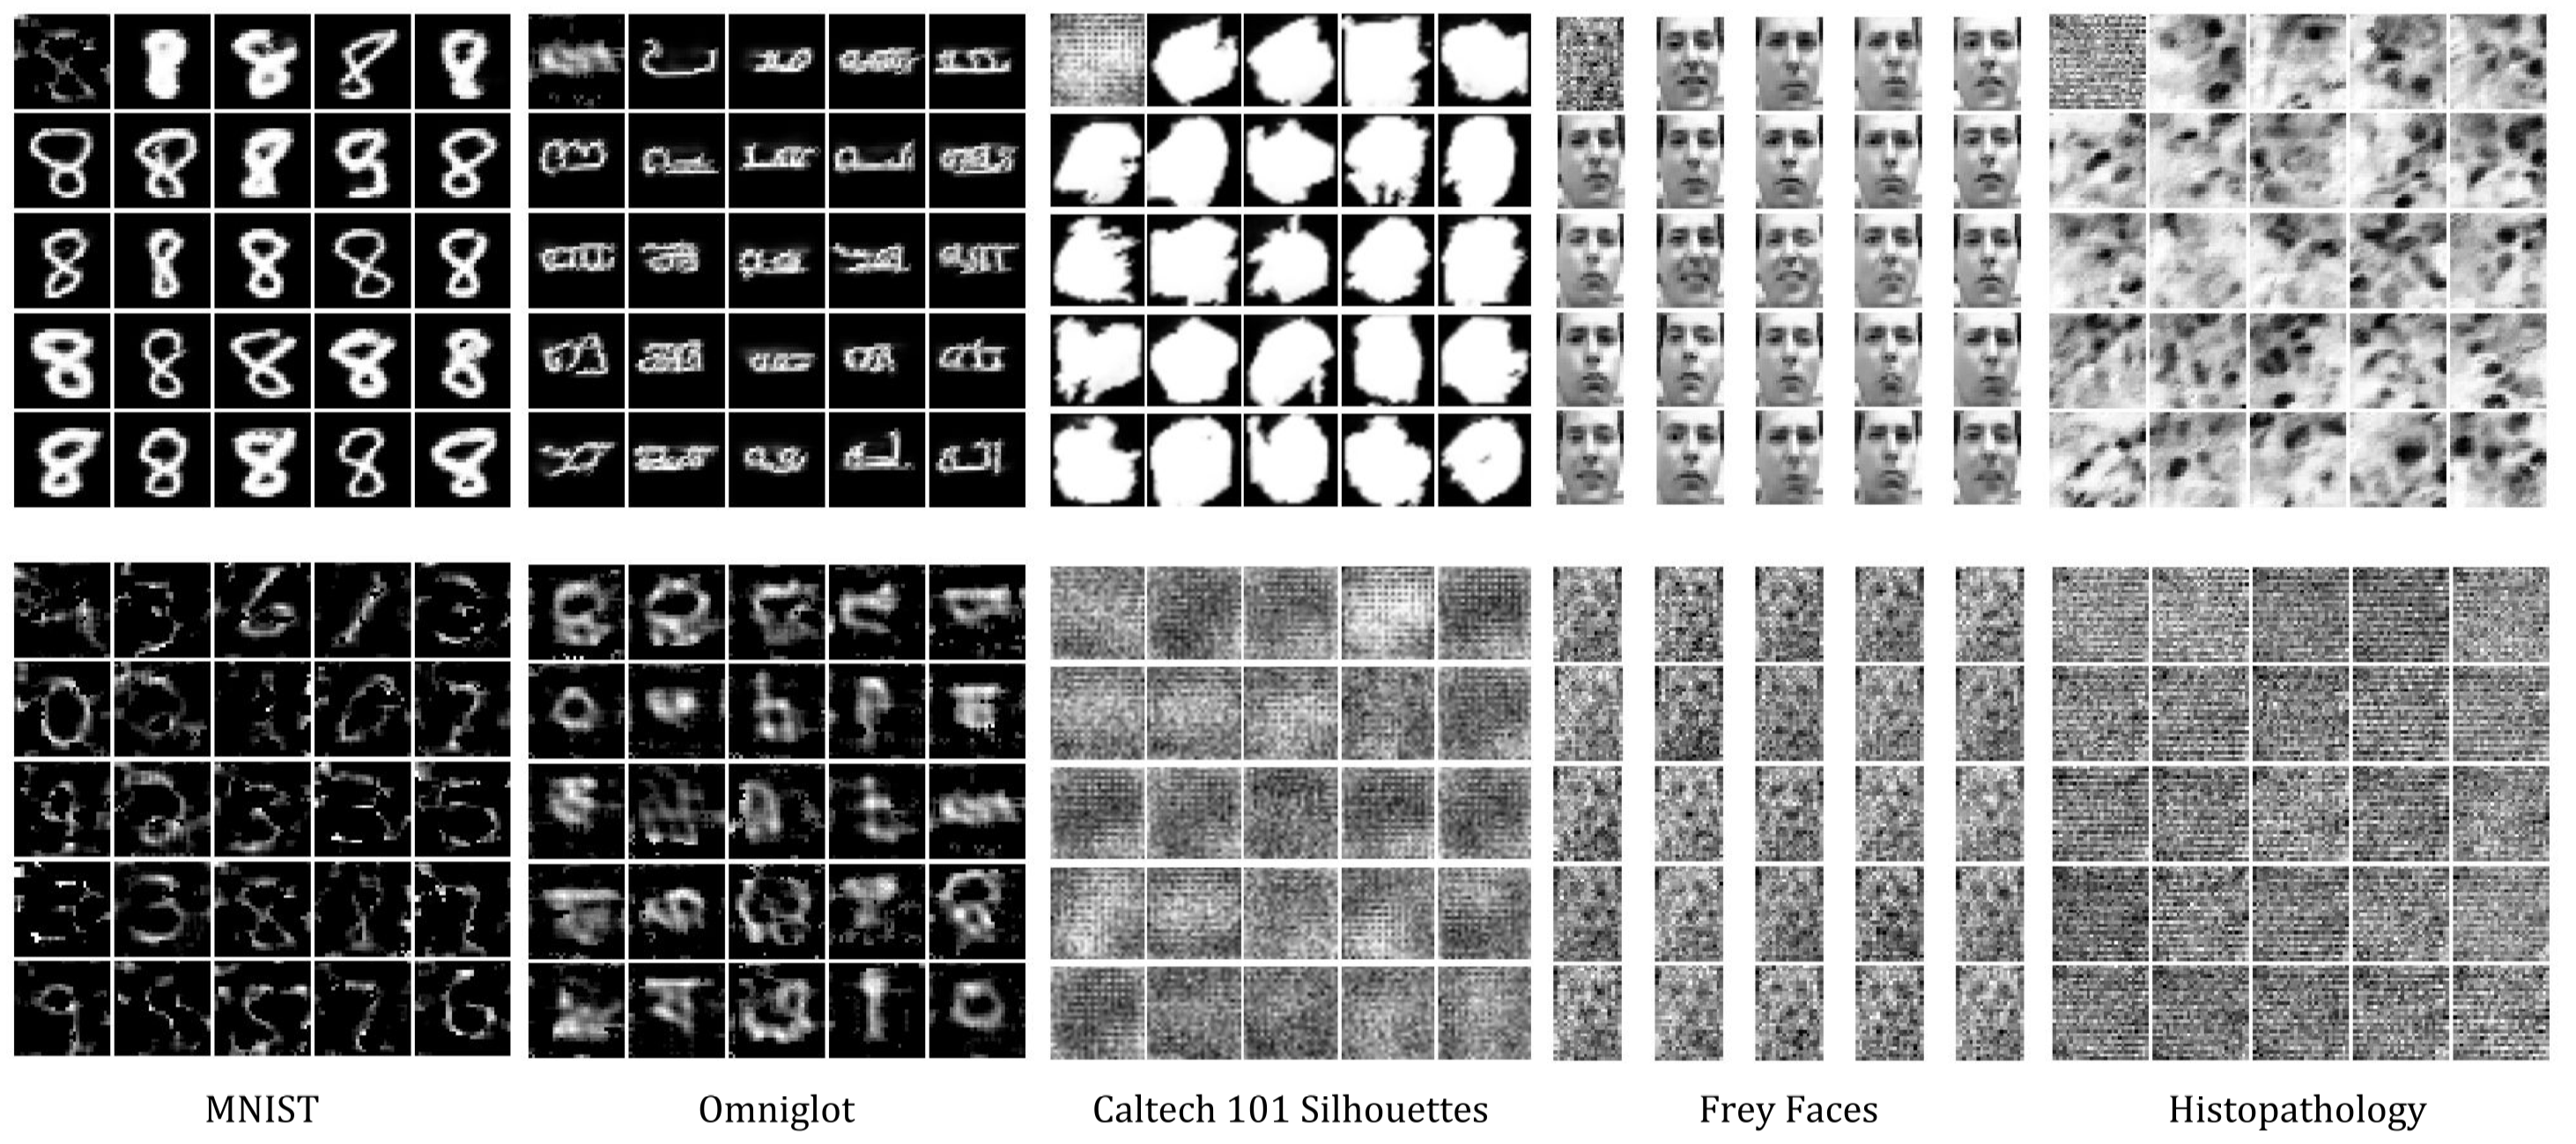
\includegraphics[width=1.0\linewidth]{figs/VampPrior_4.png}
	\end{figure}
	\vfill
	\hrule\medskip
	{\scriptsize \href{https://arxiv.org/pdf/1705.07120.pdf}{https://arxiv.org/pdf/1705.07120.pdf}}
\end{frame}
%=======
\begin{frame}{VAE limitations}
\begin{itemize}
	\item Poor variational posterior distribution (encoder)
	\[
	q(\bz | \bx, \bphi) = \mathcal{N}(\bz| \bmu_{\bphi}(\bx), \bsigma^2_{\bphi}(\bx)).
	\]
	\item Poor prior distribution
	\[
	p(\bz) = \mathcal{N}(0, \mathbf{I}).
	\]
	\item Poor probabilistic model (decoder)
	\[
	p(\bx | \bz, \btheta) = \mathcal{N}(\bx| \bmu_{\btheta}(\bz), \bsigma^2_{\btheta}(\bz)).
	\]
	\item Loose lower bound
	\[
	p(\bx | \btheta) - \mathcal{L}(q, \btheta) = (?).
	\]
\end{itemize}
\end{frame}
%=======
\begin{frame}{Posterior collapse: toy example}
	Let define latent variable model in the following way:
	\[
		p(\bx | \btheta) = \int p(\bx, \bz | \btheta) d \bz = \int p(\bx | \bz, \btheta) p(\bz) d \bz 
	\]
	\begin{itemize}
		\item prior distribution $p(\bz) = \mathcal{N}(\bz| 0, \mathbf{I})$;
		\item probabilistic model $p(\bx | \bz, \btheta) = \mathcal{N}(\bx | \bmu_{\btheta}(\bz), \bsigma_{\btheta}(\bz))$ (diagonal covariance);
		\item variational posterior $q(\bz | \bx, \bphi) =  \mathcal{N}(\bx | \bmu_{\bphi}(\bx), \bsigma_{\phi}(\bx))$  (diagonal covariance).
	\end{itemize}
	
	Let data distribution is $\pi(\bx) = \mathcal{N}(\bx | \bmu, \bSigma)$. Possible cases:
	\begin{itemize}
		\item covariance matrix $\bSigma$ is diagonal (univariate case);
		\item covariance matrix $\bSigma$ is \textbf{not} diagonal (multivariate case).
	\end{itemize}
	What is the difference?
\end{frame}
%=======
\begin{frame}{Posterior collapse: toy example}
	\begin{block}{Multivariate ($\bSigma$ is non-diagonal)}
		\vspace{-0.5cm}
		\begin{minipage}[t]{0.33\columnwidth}
			\begin{figure}[h]
				\centering
				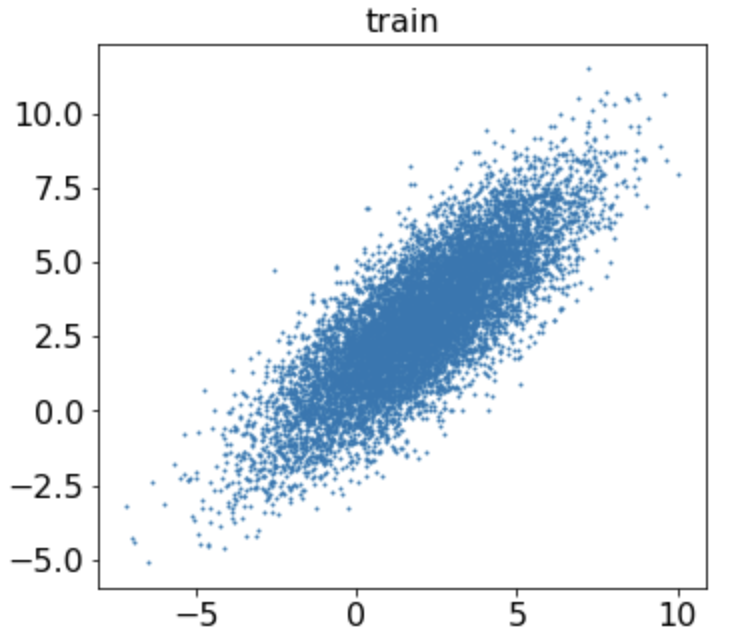
\includegraphics[width=.8\linewidth]{figs/posterior_collapse_toy_1.png}
			\end{figure}
		\end{minipage}%
		\begin{minipage}[t]{0.33\columnwidth}
			\begin{figure}[h]
				\centering
				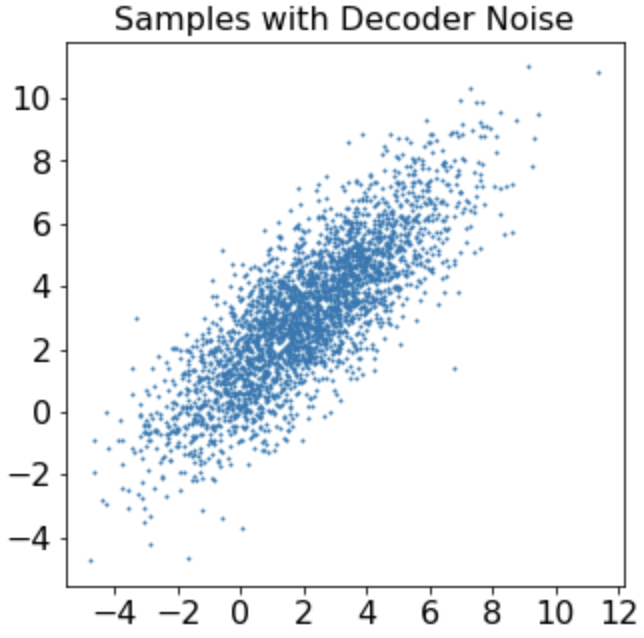
\includegraphics[width=0.75\linewidth]{figs/posterior_collapse_toy_3.png}
			\end{figure}
		\end{minipage}%
		\begin{minipage}[t]{0.33\columnwidth}
			\begin{figure}[h]
				\centering
				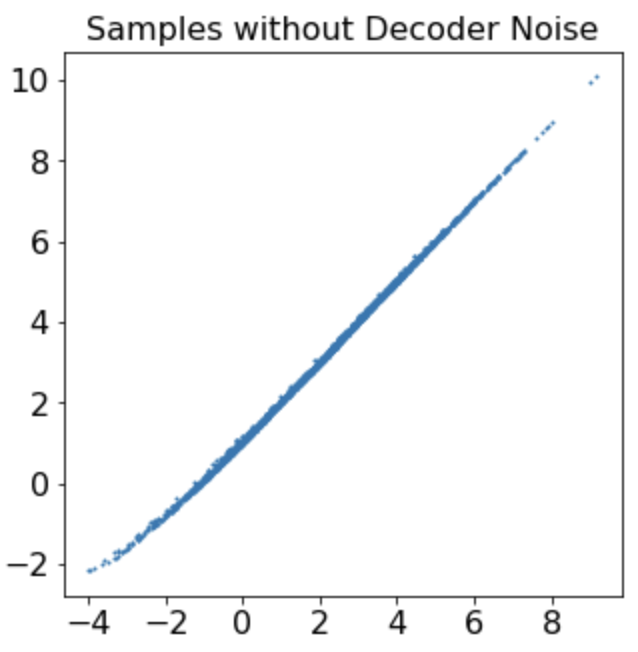
\includegraphics[width=.75\linewidth]{figs/posterior_collapse_toy_5.png}
			\end{figure}
		\end{minipage}
	The encoder uses latent variables to model data.
	\end{block}

	\begin{block}{Univariate ($\bSigma$ is diagonal)}
		\vspace{-0.5cm}
		\begin{minipage}[t]{0.33\columnwidth}
		\begin{figure}[h]
			\centering
			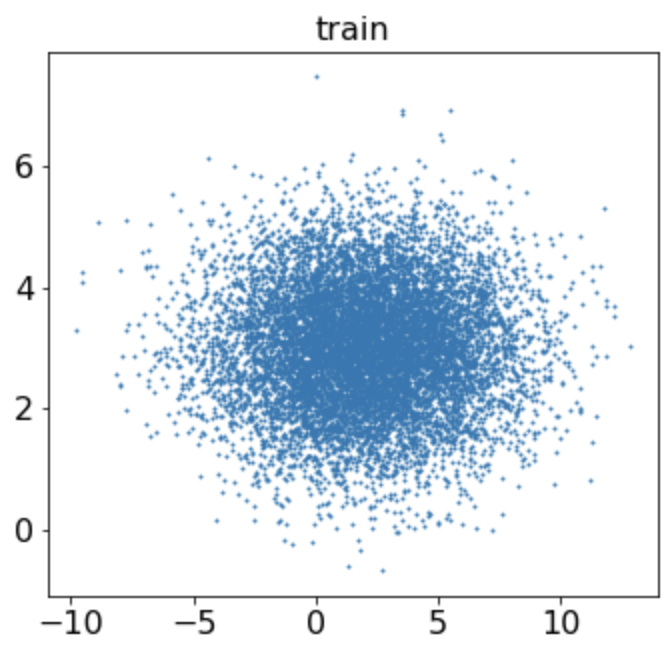
\includegraphics[width=.8\linewidth]{figs/posterior_collapse_toy_2.png}
		\end{figure}
		\end{minipage}%
		\begin{minipage}[t]{0.33\columnwidth}
		\begin{figure}[h]
			\centering
			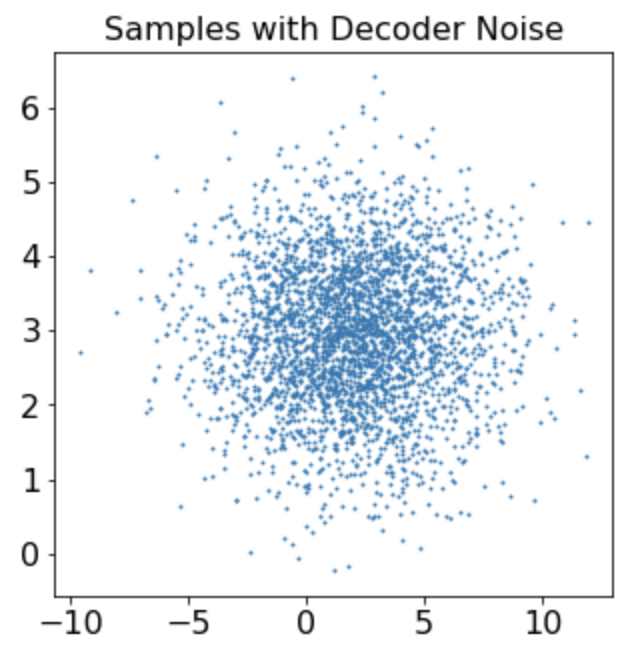
\includegraphics[width=.75\linewidth]{figs/posterior_collapse_toy_4.png}
		\end{figure}
		\end{minipage}%
		\begin{minipage}[t]{0.33\columnwidth}
		\begin{figure}[h]
			\centering
			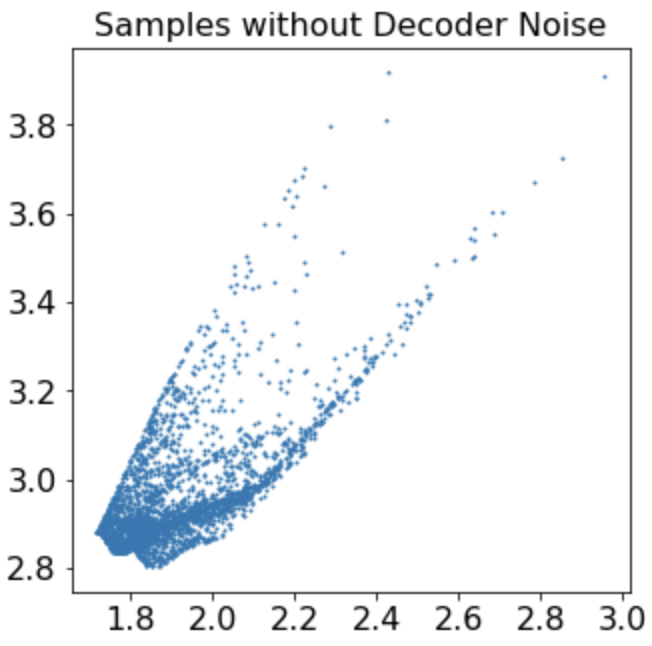
\includegraphics[width=.75\linewidth]{figs/posterior_collapse_toy_6.png}
		\end{figure}
		\end{minipage}
	Latent variables are not used, since the decoder could model the data without the encoder.
	\end{block}
\end{frame}
%=======
\begin{frame}{Posterior collapse}
	\begin{block}{Representation learning}
		"Identifies and disentangles the underlying causal factors of the data, so that it becomes easier to understand the data, to classify it, or to perform other tasks".
	\end{block}
	\[
		p(\bx | \btheta) = \int p(\bx, \bz | \btheta) d \bz = \int p(\bx | \bz, \btheta) p(\bz) d \bz 
	\]
	If the decoder model $p(\bx | \bz, \btheta)$ is powerful enough to model $p(\bx | \btheta)$ the latent variables $\bz$ becames irrelevant.
	
	\[
		\mathcal{L}(q, \btheta) = \frac{1}{n} \sum_{i=1}^n \left[ \mathbb{E}_{q(\bz_i | \bx_i)} \log p(\bx_i | \bz_i, \btheta) - KL(q(\bz_i | \bx_i) || p(\bz_i)) \right].
	\]
	Early in the training the approximate posterior $q(\bz|\bx)$ carries little information about $\bx$ and the model sets the posterior to the prior to avoid paying any cost $KL(q(\bz|\bx)||p(\bz))$.
\end{frame}
%=======
\begin{frame}{PixelVAE, 2016}
	\[
	    p(\bx | \btheta) = \int p(\bx, \bz | \btheta) d \bz = \int p(\bx | \bz, \btheta) p(\bz) d \bz 
	\]
	\begin{itemize}
		\item More powerful $p(\bx | \bz, \btheta)$ leads to more powerful generative model $p(\bx | \btheta)$.
		\item Too powerful $p(\bx | \bz, \btheta)$ could lead to posterior collapse, where variational posterior $q(\bz | \bx)$ will not carry any information about data and close to prior $p(\bz)$.
	\end{itemize}
	How to make the generative model $p(\bx | \bz, \btheta)$ more powerful?
	\begin{block}{Autoregressive decoder}
	\[
	    p(\bx | \bz , \btheta) = \prod_{i=1}^n p(x_i | \bx_{1:i - 1}, \bz , \btheta)
	\]
	\end{block}
	
	\vfill
	\hrule\medskip
	{\scriptsize \href{https://arxiv.org/pdf/1611.05013.pdf}{https://arxiv.org/pdf/1611.05013.pdf}}
\end{frame}
%=======
\begin{frame}{PixelVAE, 2016}
	VAE model with autoregressive PixelCNN decoder with few autoregressive layers. 
	\begin{itemize}
		\item Global structure is captured by latent variables.
		\item Local statistics are captured by limited receptive field autoregressive model.
	\end{itemize}
	\begin{figure}
	    \centering
	    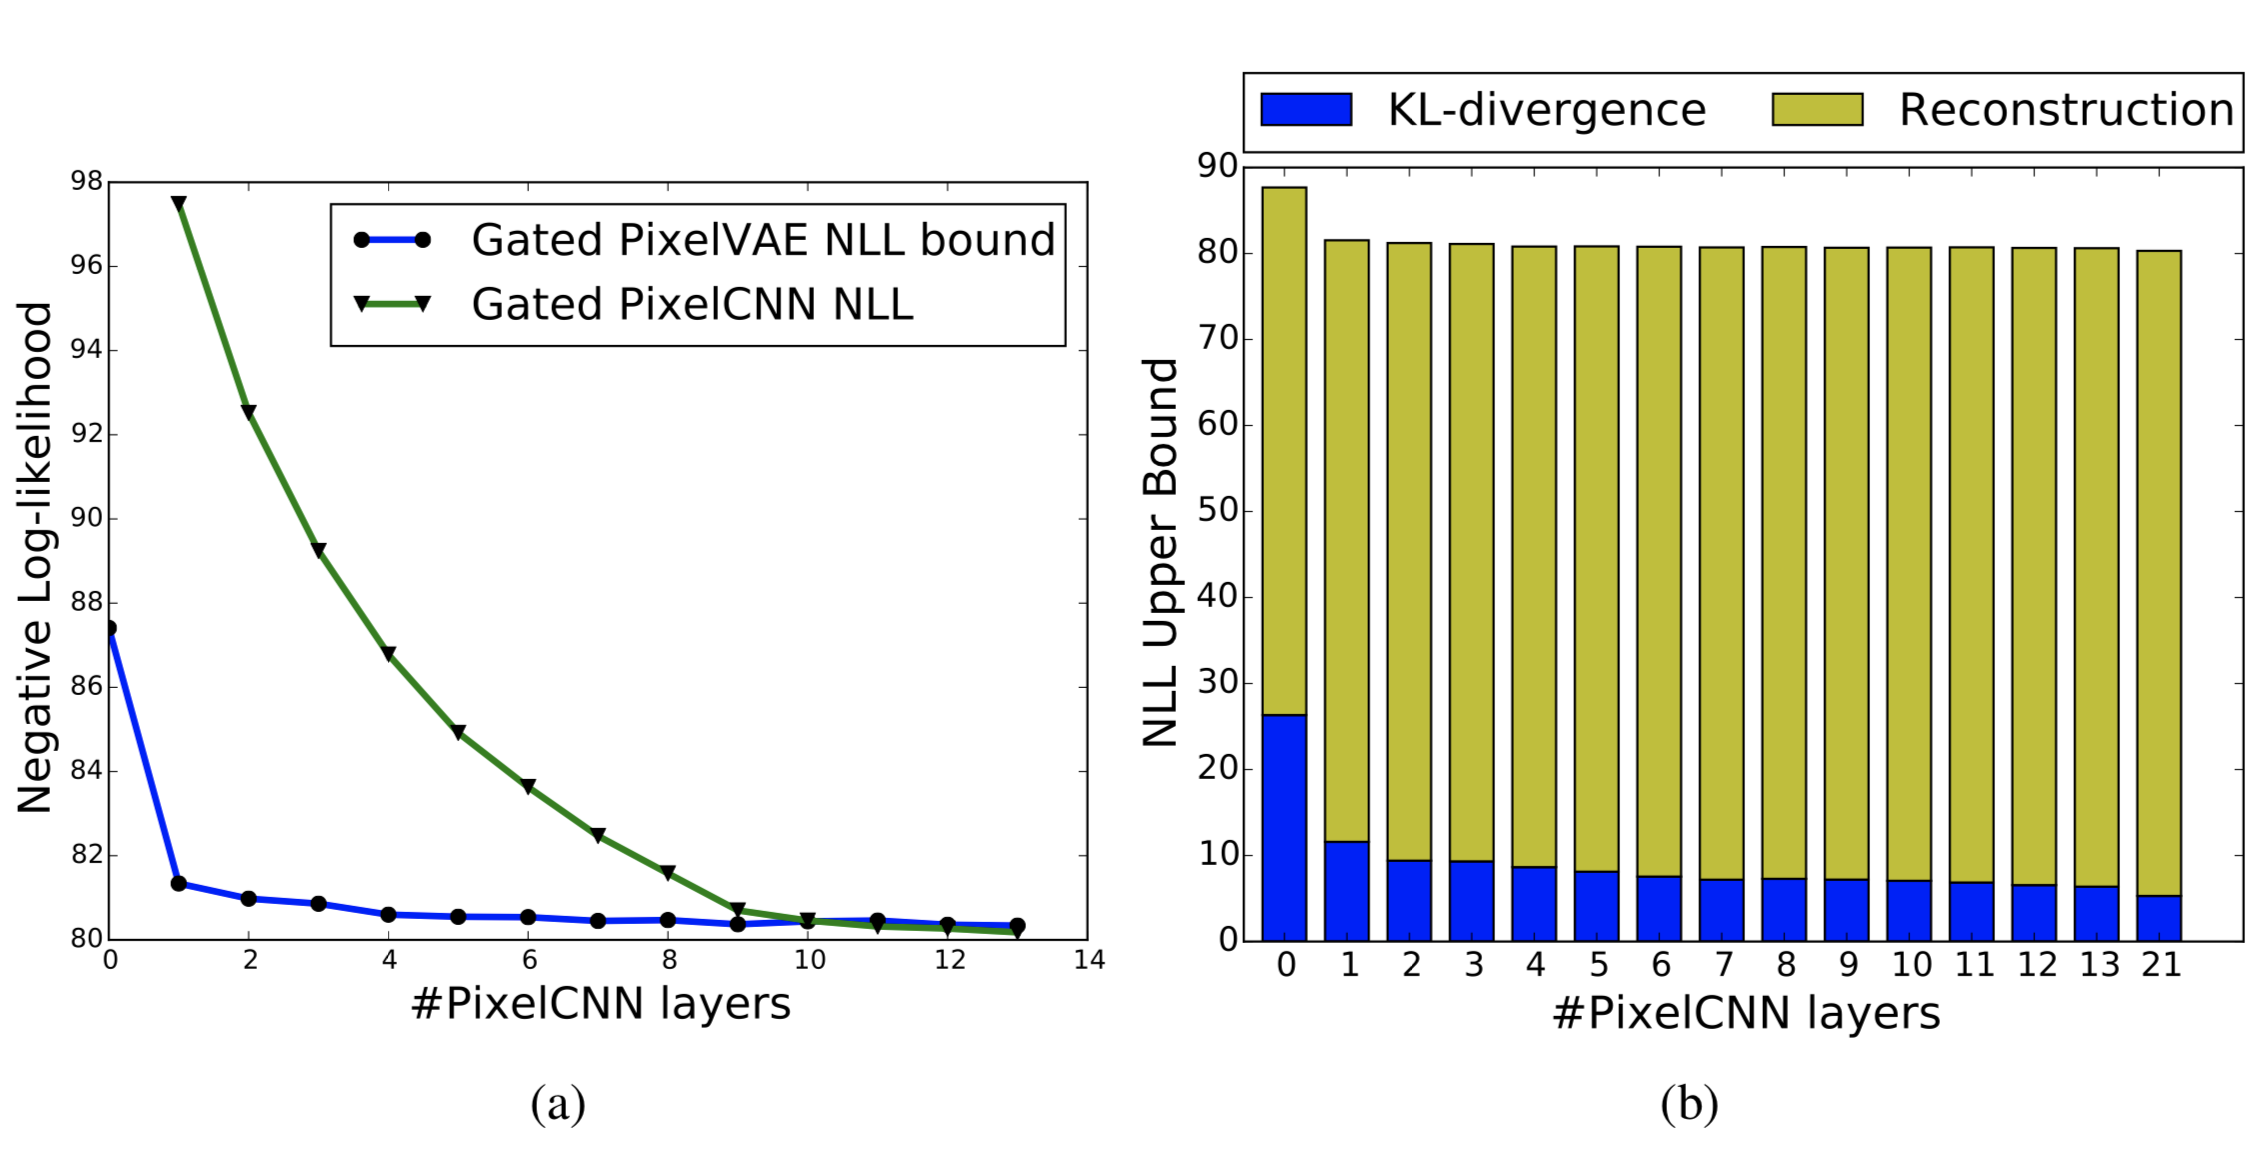
\includegraphics[width=0.8\linewidth]{figs/PixelVAE_2.png}
	\end{figure}
	\vfill
	\hrule\medskip
	{\scriptsize \href{https://arxiv.org/pdf/1611.05013.pdf}{https://arxiv.org/pdf/1611.05013.pdf}}
\end{frame}
%=======
\begin{frame}{PixelVAE, 2016}
	\begin{minipage}[t]{0.5\columnwidth}
		MNIST
		\begin{figure}
			\centering
			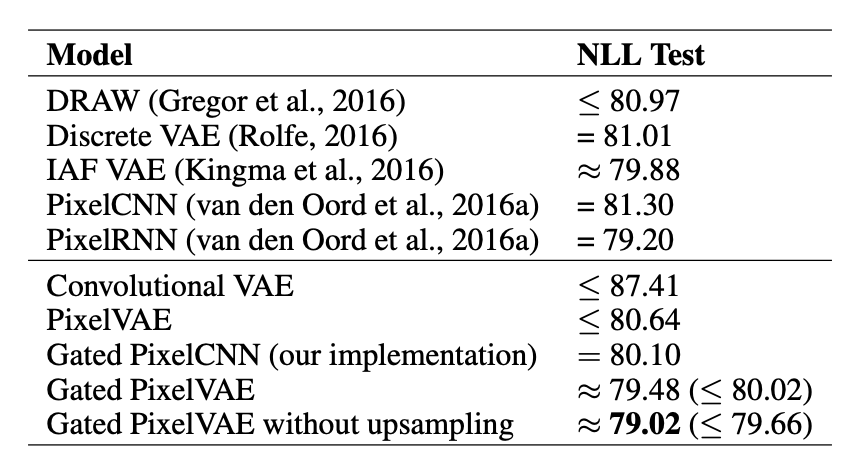
\includegraphics[width=0.9\linewidth]{figs/PixelVAE_5.png}
		\end{figure}
	\end{minipage}%
	\begin{minipage}[t]{0.5\columnwidth}
		ImageNet 64x64
		\begin{figure}
			\centering
			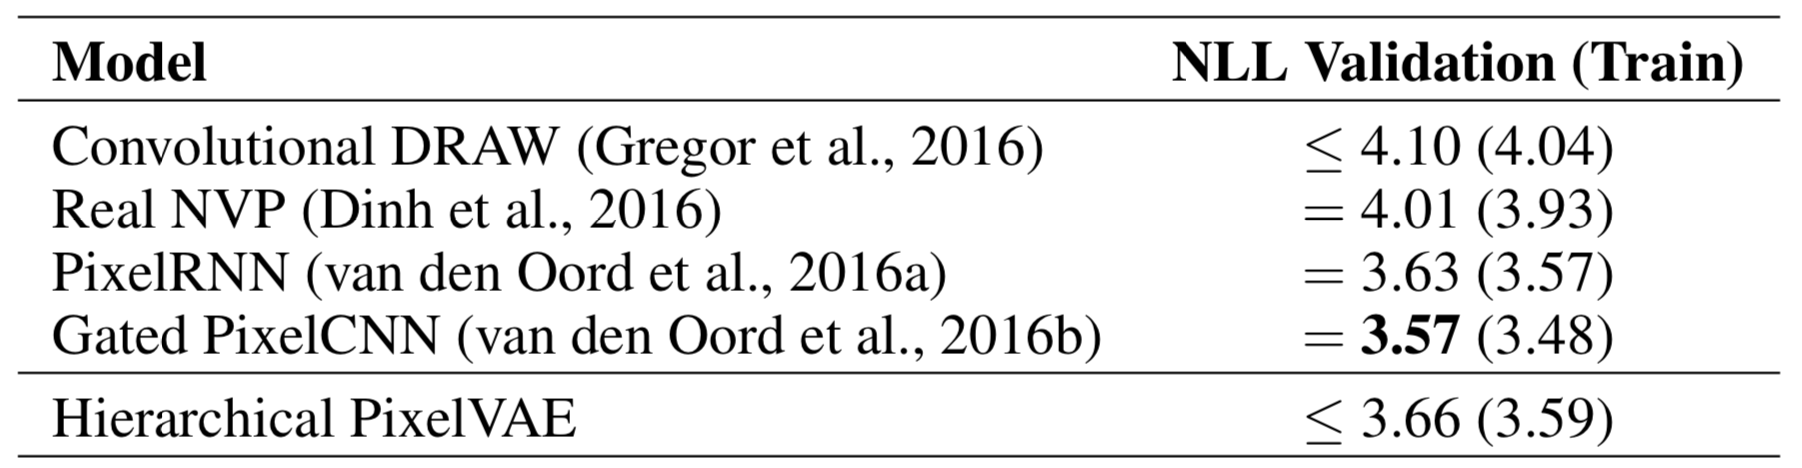
\includegraphics[width=\linewidth]{figs/PixelVAE_4.png}
		\end{figure}
	\end{minipage}
\begin{figure}
    \centering
    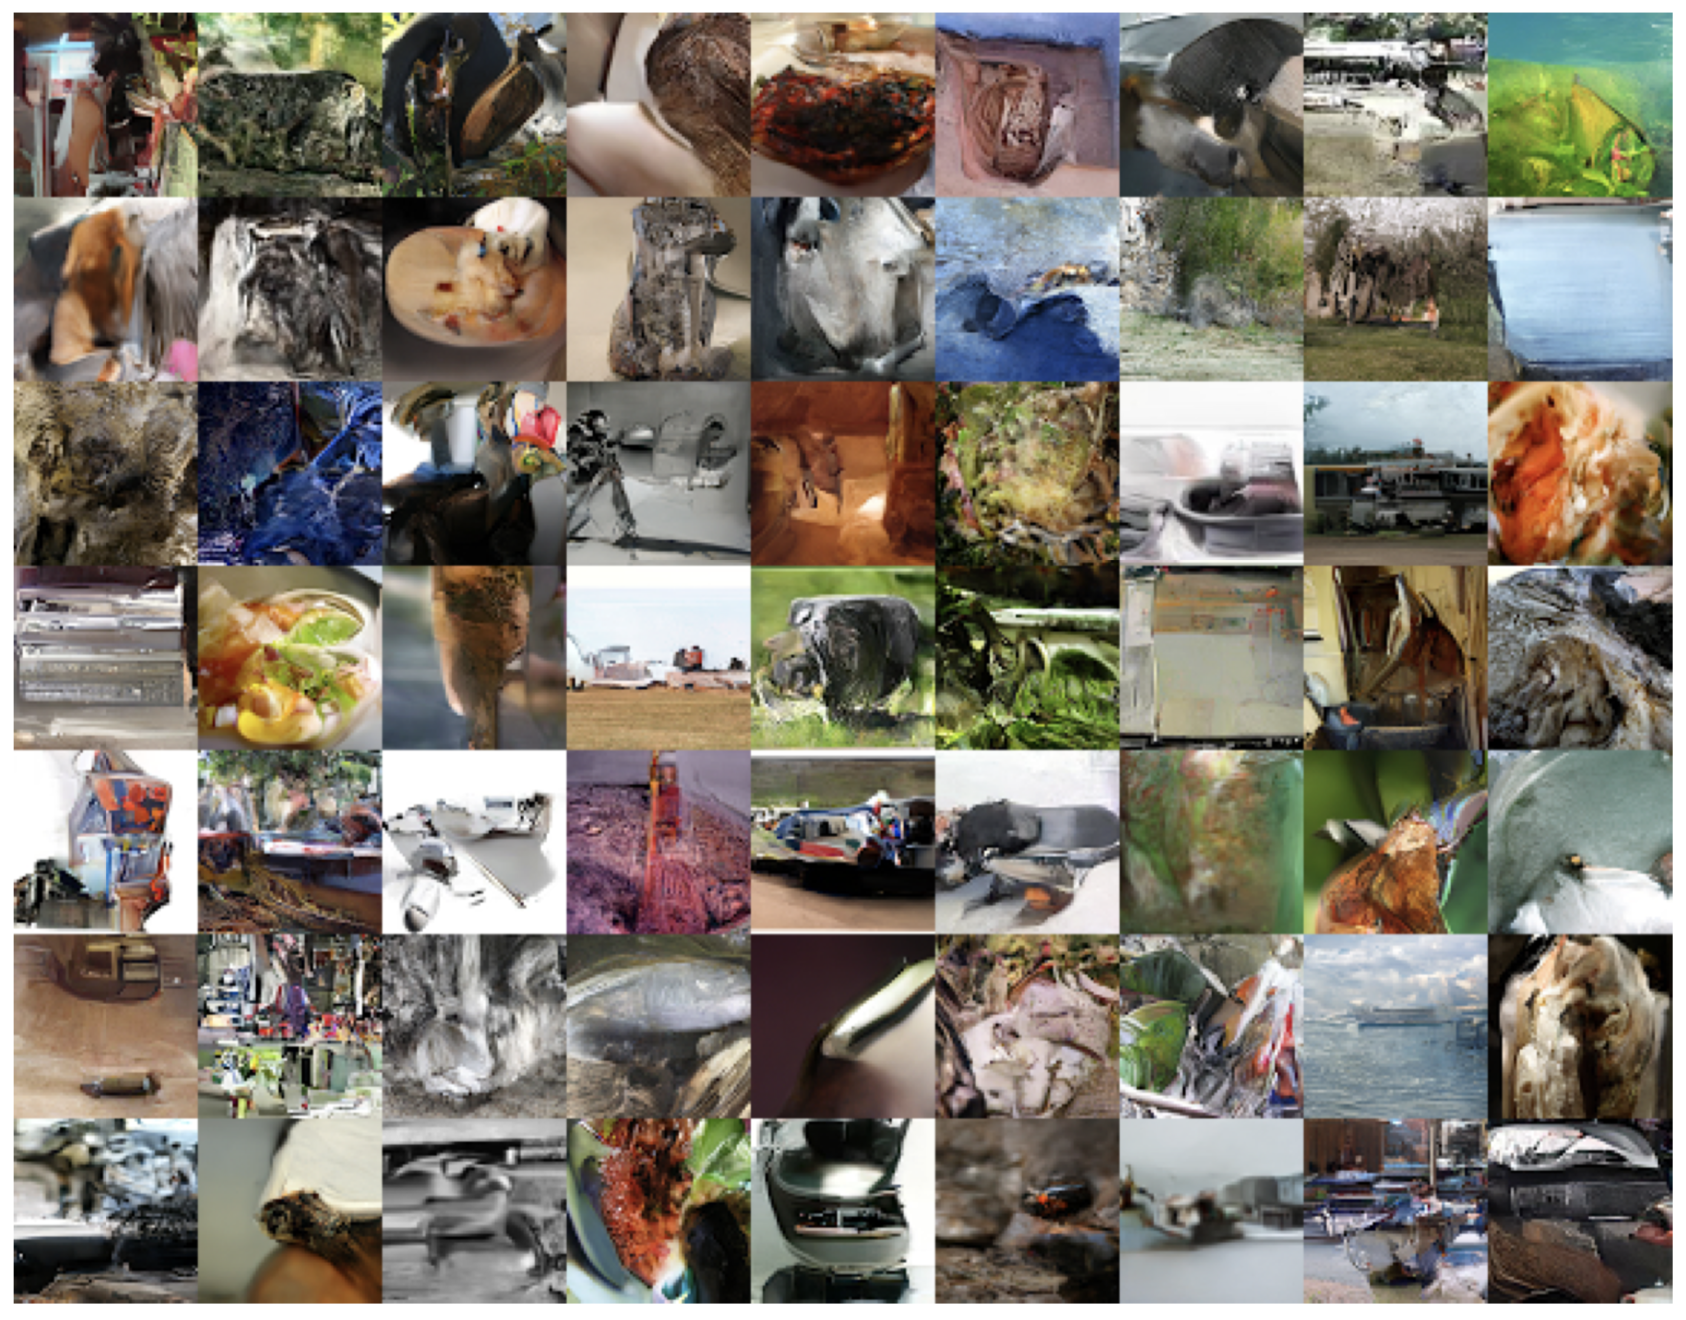
\includegraphics[width=0.5\linewidth]{figs/PixelVAE_3.png}
\end{figure}
\vfill
\hrule\medskip
{\scriptsize \href{https://arxiv.org/pdf/1611.05013.pdf}{https://arxiv.org/pdf/1611.05013.pdf}}
\end{frame}
%=======
\begin{frame}{Decoder weakening}
	\[
		p(\bx | \btheta) = \int p(\bx, \bz | \btheta) d \bz = \int p(\bx | \bz, \btheta) p(\bz) d \bz 
	\]
	Powerful decoder $p(\bx | \bz, \btheta)$ makes the model expressive, but posterior collapse is possible.
	
	PixelVAE model uses the autoregressive PixelCNN model with small number of layers to limit receptive field.
	
	How to force the model encode information about $\bx$ into $\bz$?
	\[
	    \mathcal{L}(q, \btheta) = \mathbb{E}_{q(\bz | \bx)} \log p(\bx | \bz, \btheta) - \beta \cdot KL (q(\bz | \bx) || p(\bz))
	\]
	What we get if $\beta = 1$ ($\beta = 0$)? \\
	
	\begin{block}{KL annealing}
		\begin{itemize}
		    \item Start training with $\beta = 0$.
		    \item Increase it until $\beta = 1$ during training process.
		\end{itemize}
	\end{block}
	\vfill
	\hrule\medskip
	{\scriptsize \href{https://arxiv.org/abs/1511.06349}{https://arxiv.org/abs/1511.06349}}
\end{frame}
%=======
\begin{frame}{Decoder weakening}
\begin{block}{Free bits}
\begin{itemize}
\item Divide the latent dimensions into the $K$ subsets.
\item Ensure that using less than $\lambda$ nats of information per subset $j$.
\end{itemize}

\[
    \hat{\mathcal{L}}(q, \btheta) = \mathbb{E}_{q(\bZ | \bX)} \log p(\bX | \bZ, \btheta) - \sum_{j=1}^K \max(\lambda, KL (q(\bZ_j | \bX) || p(\bZ_j))).
\]

Increasing the latent information is advantageous for the reconstruction term. \\
\vspace{0.2cm}
This results in $KL (q(\bZ_j | \bx) || p(\bZ_j)) \geq \lambda$ for all $j$, in practice.
\end{block}
\vspace{1cm}
\vfill
\hrule\medskip
{\scriptsize \href{https://arxiv.org/abs/1606.04934}{https://arxiv.org/abs/1606.04934}}
\end{frame}
%=======
\begin{frame}{Variational Lossy AutoEncoder, 2016}
\begin{block}{Lossy code via explicit information placement}
\[
    p(\bx | \bz, \btheta) = \prod_{i=1}^m p(x_i | \bz, \bx_{\text{WindowAround}(i)}, \btheta).
\]
\begin{itemize}
    \item WindowAround($i$) restricts the receptive field (it forbids to represent arbitrarily complex distribution over $\bx$ without dependence on $\bz$). 
    \item Local statistics of 2D images (texture) will be modeled by a small local window.
    \item Global structural information (shapes) is long-range dependency that can only be communicated through latent code $\bz$. 
\end{itemize}
\end{block}
\vspace{0.7cm}
\vfill
\hrule\medskip
{\scriptsize \href{https://arxiv.org/abs/1606.04934}{https://arxiv.org/abs/1606.04934}}
\end{frame}
%=======
\begin{frame}{Variational Lossy AutoEncoder, 2016}
	
	\begin{block}{ELBO revisiting}
		\vspace{-0.3cm}
		{\footnotesize
			\[
			\mathcal{L}(q, \btheta) = \underbrace{\frac{1}{n} \sum_{i=1}^n \mathbb{E}_{q(\bz_i | \bx_i)} \log p(\bx_i | \bz_i, \btheta)}_{\text{Reconstruction loss}} - \underbrace{\left(\log n - \mathbb{E}_{q(\bz)} \mathbb{H} \left[ q(i | \bz) \right] \right)\vphantom{\sum_{i=1}}}_{0 \leq \text{Mutual info} \leq \log N } - \underbrace{KL(q(\bz) || p(\bz))\vphantom{\sum_{i=1}}}_{\text{Marginal KL}}
			\]}
	\end{block}
	\vspace{-0.5cm}
	\begin{block}{VampPrior}
		\vspace{-0.5cm}
		\[
			p(\bz | \blambda) = \frac{1}{K} \sum_{k=1}^K q(\bz | \bu_k),
		\]
	where $\bu_1, \dots \bu_K$ is trainable preudo-inputs.
	\end{block}
	\begin{block}{Autoregressive flow prior}
		\vspace{-0.5cm}
		\[
			\log p(\bz | \blambda) = \log p(\bepsilon) + \log \det \left | \frac{d \bepsilon}{d\bz}\right|
		\]
		\[
			\bz = g(\bepsilon, \blambda) = f^{-1}(\bepsilon, \blambda) 
		\]
	\end{block}
	\vfill
	\hrule\medskip
	{\scriptsize \href{https://arxiv.org/abs/1606.04934}{https://arxiv.org/abs/1606.04934}}
\end{frame}
%=======
\begin{frame}{Variational Lossy AutoEncoder, 2016}
\begin{block}{Theorem}
VAE with AF prior in latent code $\bz$ is equivalent to using IAF posterior for latent code $\bepsilon$.
\end{block}
\begin{block}{Proof}
\vspace{-0.5cm}
{\footnotesize
\begin{align*}
\mathcal{L}(q, \btheta) &= \mathbb{E}_{q(\bz | \bx)} \left[ \log p(\bx | \bz, \btheta) +  \log p(\bz, \blambda) - q(\bz | \bx) \right] \\
&= \mathbb{E}_{\bz \sim q(\bz | \bx)} \Bigl[ \log p(\bx | \bz, \btheta) + \underbrace{ \Bigl( \log p(f(\bz, \blambda)) + \log \left| \det \frac{\partial f(\bz, \blambda)}{\partial \bz} \right| \Bigr) }_{\text{AF prior}} - q(\bz | \bx) \Bigr] \\
&= \mathbb{E}_{\bz \sim q(\bz | \bx)} \Bigl[ \log p(\bx | \bz, \btheta) +  \log p(f(\bz, \blambda)) - \underbrace{ \Bigl( q(\bz | \bx) - \log \left| \det \frac{\partial f(\bz, \blambda)}{\partial \bz} \right| \Bigr) }_{\text{IAF posterior}} \Bigr]
\end{align*}
}
\end{block}
\vfill
\hrule\medskip
{\scriptsize \href{https://arxiv.org/abs/1606.04934}{https://arxiv.org/abs/1606.04934}}
\end{frame}
%=======
\begin{frame}{Variational Lossy AutoEncoder, 2016}
	\begin{block}{Autoregressive flow prior}
		{\footnotesize
		\begin{align*}
			\mathcal{L}(q, \btheta) &= \mathbb{E}_{\bz \sim q(\bz | \bx)} \Bigl[ \log p(\bx | \bz, \btheta) + \underbrace{ \Bigl( \log p(f(\bz, \blambda)) + \log \left| \det \frac{\partial f(\bz, \blambda)}{\partial \bz} \right| \Bigr) }_{\text{AF prior}} - q(\bz | \bx) \Bigr] \\
			&= \mathbb{E}_{\bz \sim q(\bz | \bx)} \Bigl[ \log p(\bx | \bz, \btheta) +  \log p(f(\bz, \blambda)) - \underbrace{ \Bigl( q(\bz | \bx) - \log \left| \det \frac{\partial f(\bz, \blambda)}{\partial \bz} \right| \Bigr) }_{\text{IAF posterior}} \Bigr]
		\end{align*}
		}
	\end{block}
	\begin{itemize}
		\item IAF posterior decoder path: $p(\bx|\bz, \btheta)$, $\bz \sim p(\bz)$.
		\item AF prior decoder path: $p(\bx|\bz, \btheta)$, $\bz = g(\bepsilon, \blambda)$, $\bepsilon \sim p(\bepsilon)$. 
	\end{itemize}
	AF prior and IAF posterior have the same computation cost, so using AF prior makes the model more expressive at no training time cost.
\vfill
\hrule\medskip
{\scriptsize \href{https://arxiv.org/abs/1606.04934}{https://arxiv.org/abs/1606.04934}}
\end{frame}
%=======
\begin{frame}{Variational Lossy AutoEncoder, 2016}
\begin{itemize}
    \item Can VLAE learn lossy codes that encode global statistics?
    \item Does using AF priors improves upon using IAF posteriors as predicted by theory?
    \item Does using autoregressive decoding distributions improve density estimation performance?
\end{itemize}
	\begin{minipage}[t]{0.5\columnwidth}
	\vspace{1cm}
		MNIST
		\begin{figure}[h]
			\centering
			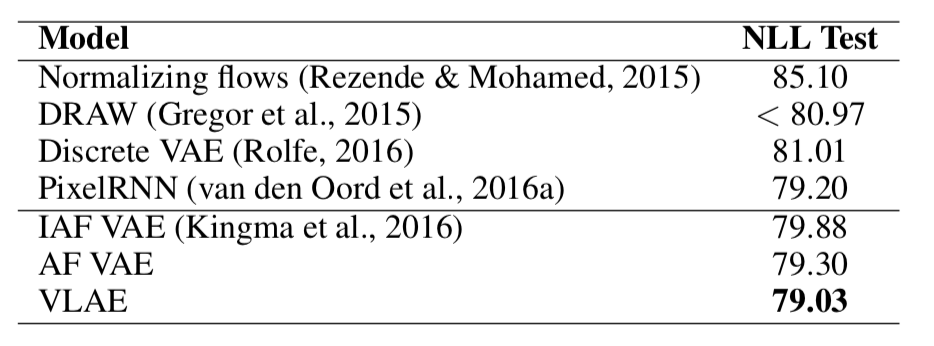
\includegraphics[width=1.\linewidth]{figs/VLAE_1.png}
		\end{figure}
	\end{minipage}%
	\begin{minipage}[t]{0.5\columnwidth}
		CIFAR10
		\begin{figure}[h]
			\centering
			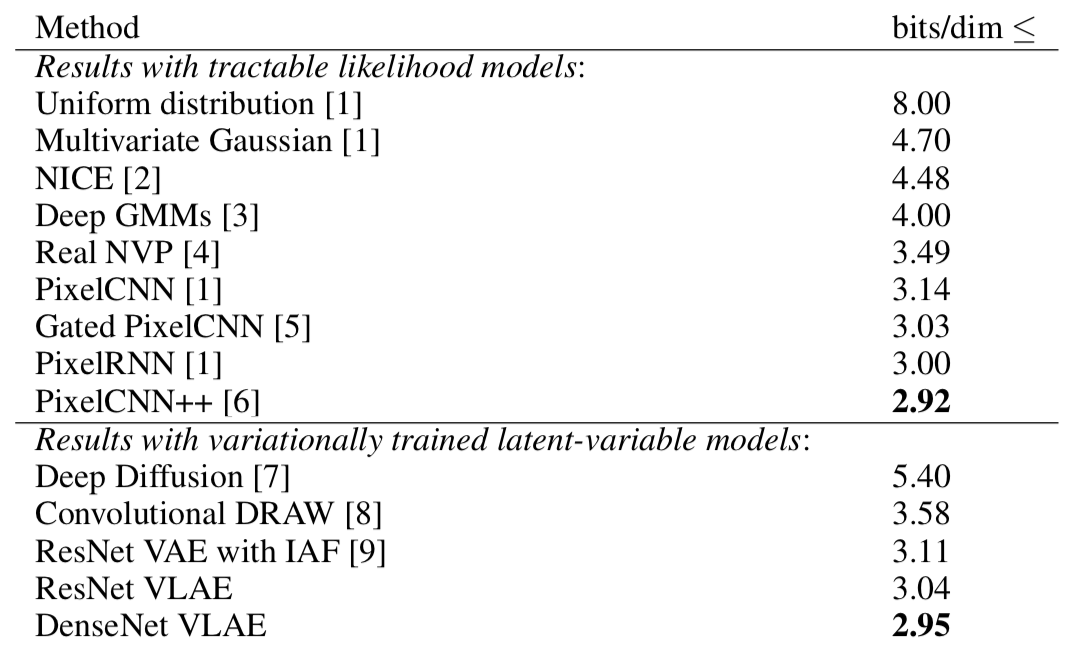
\includegraphics[width=1.\linewidth]{figs/VLAE_2.png}
		\end{figure}
	\end{minipage}
\vfill
\hrule\medskip
{\scriptsize \href{https://arxiv.org/abs/1606.04934}{https://arxiv.org/abs/1606.04934}}
\end{frame}
%=======
\begin{frame}{VAE limitations}
	\begin{itemize}
		\item Poor variational posterior distribution (encoder)
		\[
		q(\bz | \bx, \bphi) = \mathcal{N}(\bz| \bmu_{\bphi}(\bx), \bsigma^2_{\bphi}(\bx)).
		\]
		\item Poor prior distribution
		\[
		p(\bz) = \mathcal{N}(0, \mathbf{I}).
		\]
		\item Poor probabilistic model (decoder)
		\[
		p(\bx | \bz, \btheta) = \mathcal{N}(\bx| \bmu_{\btheta}(\bz), \bsigma^2_{\btheta}(\bz)).
		\]
		\item Loose lower bound
		\[
		p(\bx | \btheta) - \mathcal{L}(q, \btheta) = (?).
		\]
	\end{itemize}
\end{frame}
%=======
\begin{frame}{Importance Sampling}
	\begin{block}{Generative model}
		\vspace{-0.5cm}
		\begin{align*}
			p(\bx | \btheta) &= \int p(\bx, \bz | \btheta) d\bz = \int \left[\frac{p(\bx, \bz | \btheta)}{q(\bz | \bx)} \right] q(\bz | \bx) d\bz \\
			&= \int f(\bx, \bz) q(\bz | \bx) d\bz = \mathbb{E}_{\bz \sim q(\bz | \bx)} f(\bx, \bz)
		\end{align*}
	\end{block}
	Here $f(\bx, \bz) = \frac{p(\bx, \bz | \btheta)}{q(\bz | \bx)}$.
	\begin{block}{ELBO}
		\vspace{-0.5cm}
		\begin{multline*}
			\log p(\bx | \btheta) = \log \mathbb{E}_{\bz \sim q(\bz | \bx)} f(\bx, \bz)
			\geq \mathbb{E}_{\bz \sim q(\bz | \bx)} \log f(\bx, \bz) = \\
			= \mathbb{E}_{\bz \sim q(\bz | \bx)} \log \frac{p(\bx, \bz | \btheta)}{q(\bz | \bx)} = \mathcal{L}(q, \btheta).
		\end{multline*}
	\end{block}
	Could we choose better $f(\bx, \bz)$? 
\end{frame}
%=======
\begin{frame}{IWAE, 2015}
	Let define
	\[
	f(\bx, \bz_1, \dots, \bz_K) = \frac{1}{K} \sum_{k=1}^K \frac{p(\bx, \bz_k | \btheta)}{q(\bz_k | \bx)}
	\]
	\[
		\mathbb{E}_{\bz_1, \dots, \bz_K \sim q(\bz | \bx)} f(\bx, \bz_1, \dots, \bz_K) = p(\bx | \btheta)
	\]
	\vspace{-0.3cm}
	\begin{block}{ELBO}
		\vspace{-0.5cm}
		\begin{multline*}
			\log p(\bx | \btheta) = \log \mathbb{E}_{\bz_1, \dots, \bz_K \sim q(\bz | \bx)} f(\bx, \bz, \dots, \bz_K) \geq \\
			\geq \mathbb{E}_{\bz_1, \dots, \bz_K \sim q(\bz | \bx)} \log f(\bx, \bz, \dots, \bz_K) = \\
			= \mathbb{E}_{\bz_1, \dots, \bz_K \sim q(\bz | \bx)} \log \left[\frac{1}{K} \sum_{k=1}^K\frac{p(\bx, \bz_k | \btheta)}{q(\bz_k | \bx)} \right] = \mathcal{L}_K(q, \btheta).
		\end{multline*}
	\end{block}
	\vfill
	\hrule\medskip
	{\scriptsize \href{https://arxiv.org/pdf/1509.00519.pdf}{https://arxiv.org/pdf/1509.00519.pdf}}
\end{frame}
%=======
\begin{frame}{IWAE, 2015}
\begin{block}{VAE objective}
	\vspace{-0.2cm}
	\[
	p(\bx | \btheta) \geq \mathcal{L} (q, \btheta)  = \mathbb{E}_{q(\bz | \bx)} \log \frac{p(\bx, \bz | \btheta)}{q(\bz| \bx)} \rightarrow \max_{\bphi, \btheta}
	\]
	\[
	\mathcal{L} (q, \btheta)  = \mathbb{E}_{\bz_1, \dots, \bz_K \sim q(\bz | \bx)} \left( \frac{1}{K} \sum_{k=1}^K \log \frac{p(\bx, \bz_k | \btheta)}{q(\bz_k| \bx)} \right) \rightarrow \max_{q, \btheta}.
	\]
	\vspace{-0.2cm}
\end{block}
\begin{block}{IWAE objective}
	\vspace{-0.2cm}
	\[
	\mathcal{L}_K (q, \btheta)  = \mathbb{E}_{\bz_1, \dots, \bz_K \sim q(\bz | \bx)} \log \left( \frac{1}{K}\sum_{k=1}^K\frac{p(\bx, \bz_k | \btheta)}{q(\bz_k| \bx)} \right) \rightarrow \max_{q, \btheta}.
	\]
\end{block}
If $K=1$, these objectives coincide.

\vfill
\hrule\medskip
{\scriptsize \href{https://arxiv.org/pdf/1509.00519.pdf}{https://arxiv.org/pdf/1509.00519.pdf}}
\end{frame}
%=======
\begin{frame}{IWAE, 2015}
\begin{block}{Theorem}
	\begin{enumerate}
		\item $\log p(\bx | \btheta) \geq \mathcal{L}_K (q, \btheta) \geq \mathcal{L}_M (q, \btheta), \quad \text{for } K \geq M$;
		\item $\log p(\bx | \btheta) = \lim_{K \rightarrow \infty} \mathcal{L}_K (q, \btheta)$ if $\frac{p(\bx, \bz | \btheta)}{q(\bz | \bx)}$ is bounded.
	\end{enumerate}
	\vspace{-0.2cm}
\end{block}
\begin{block}{Proof of 1.}
	{ \footnotesize
		\vspace{-0.5cm}
		\begin{align*}
			\mathcal{L}_K (q, \btheta) &= \mathbb{E}_{\bz_1, \dots, \bz_K} \log \left( \frac{1}{K}\sum_{k=1}^K\frac{p(\bx, \bz_k | \btheta)}{q(\bz_k| \bx)} \right) = \\
			&= \mathbb{E}_{\bz_1, \dots, \bz_K} \log \mathbb{E}_{k_1, \dots, k_M} \left( \frac{1}{M}\sum_{m=1}^M\frac{p(\bx, \bz_{k_m} | \btheta)}{q(\bz_{k_m}| \bx)} \right) \geq \\
			&\geq \mathbb{E}_{\bz_1, \dots, \bz_K} \mathbb{E}_{k_1, \dots, k_m} \log \left( \frac{1}{M}\sum_{m=1}^M\frac{p(\bx, \bz_{k_m} | \btheta)}{q(\bz_{k_m}| \bx)} \right) = \\
			&= \mathbb{E}_{\bz_1, \dots, \bz_M} \log \left( \frac{1}{M}\sum_{m=1}^M\frac{p(\bx, \bz_m | \btheta)}{q(\bz_m| \bx)} \right) = \mathcal{L}_M (q, \btheta)
		\end{align*}
	}
\end{block}

\vfill
\hrule\medskip
{\scriptsize \href{https://arxiv.org/pdf/1509.00519.pdf}{https://arxiv.org/pdf/1509.00519.pdf}}
\end{frame}
%=======
\begin{frame}{IWAE, 2015}
\begin{block}{Theorem}
	\begin{enumerate}
		\item $\log p(\bx | \btheta) \geq \mathcal{L}_K (q, \btheta) \geq \mathcal{L}_M (q, \btheta), \quad \text{for} K \geq M$;
		\item $\log p(\bx | \btheta) = \lim_{K \rightarrow \infty} \mathcal{L}_K (q, \btheta)$ if $\frac{p(\bx, \bz | \btheta)}{q(\bz | \bx)}$ is bounded.
	\end{enumerate}
	\vspace{-0.2cm}
\end{block}
\begin{block}{Proof of 2.}
	\vspace{0.2cm}
	Consider r.v. $\xi_K = \frac{1}{K}\sum_{k=1}^K \frac{p(\bx, \bz_k | \btheta)}{q(\bz_k | \bx)}$. \\
	\vspace{0.2cm}
	If summands are bounded, then (from the strong law of large numbers)
	\[
	\xi_K \xrightarrow[K \rightarrow \infty]{a.s.} \mathbb{E}_{q(\bz | \bx)} \frac{p(\bx, \bz | \btheta)}{q(\bz | \bx)} = p(\bx | \btheta).
	\]
	Hence $\mathcal{L}_K (q, \btheta) = \mathbb{E} \log \xi_K$ converges to $\log p(\bx | \btheta)$ as $K \rightarrow \infty$.
\end{block}
\vfill
\hrule\medskip
{\scriptsize \href{https://arxiv.org/pdf/1509.00519.pdf}{https://arxiv.org/pdf/1509.00519.pdf}}
\end{frame}
%=======
\begin{frame}{IWAE, 2015}
\[
\log p(\bx | \btheta) \geq \mathcal{L}_K(q, \btheta) \geq \mathcal{L}(q, \btheta)
\]
If $K > 1$ the bound could be tighter.
\begin{align*}
	\mathcal{L} (q, \btheta) &= \mathbb{E}_{q(\bz | \bx)} \log \frac{p(\bx, \bz | \btheta)}{q(\bz| \bx)}; \\
	\mathcal{L}_K (q, \btheta) &= \mathbb{E}_{\bz_1, \dots, \bz_K \sim q(\bz | \bx)} \log \left( \frac{1}{K}\sum_{k=1}^K\frac{p(\bx, \bz_k | \btheta)}{q(\bz_k| \bx)} \right).
\end{align*}
\vspace{-0.2cm}
\begin{itemize}
	\item $\mathcal{L}_1(q, \btheta) = \mathcal{L}(q, \btheta)$;
	\item $\mathcal{L}_{\infty}(q, \btheta) = \log p(\bx | \btheta)$.
\end{itemize}
\vspace{0.2cm}
Which $q(\bz | \bx)$ gives $\mathcal{L}(q, \btheta) = \log p(\bx | \btheta)$? \\
\vspace{0.2cm}
Which $q(\bz | \bx)$ gives $\mathcal{L}(q, \btheta) = \mathcal{L}_K(q, \btheta)$?
\vfill
\hrule\medskip
{\scriptsize \href{https://arxiv.org/pdf/1509.00519.pdf}{https://arxiv.org/pdf/1509.00519.pdf}}
\end{frame}
%=======
\begin{frame}{IWAE, 2017}
\begin{block}{Theorem}
	The VAE objective is equal to IWAE objective 
	\[
	\mathcal{L}(q_{EW}, \btheta) = \mathcal{L}_K(q, \btheta)
	\]
	for the following variational distribution
	\[
	q_{EW}(\bz | \bx) = \mathbb{E}_{\bz_2, \dots, \bz_K \sim q(\bz | \bx)} q_{IW}(\bz | \bx, \bz_{2:K}),
	\]
	where \[
	q_{IW}(\bz | \bx, \bz_{2:K}) = \frac{\frac{p(\bx, \bz)}{q(\bz | \bx)})}{\frac{1}{K} \sum_{k=1}^K \frac{p(\bx, \bz_k)}{q(\bz_k | \bx)}} q(\bz | \bx) = \frac{p(\bx, \bz)}{\frac{1}{K}\left( \frac{p(\bx, \bz)}{q(\bz | \bx)} + \sum_{k=2}^K \frac{p(\bx, \bz_k)}{q(\bz_k | \bx)}\right)}.
	\]
\end{block}

\vfill
\hrule\medskip
{\scriptsize \href{https://openreview.net/pdf?id=Syw2ZgrFx}{https://openreview.net/pdf?id=Syw2ZgrFx}}
\end{frame}
%=======
\begin{frame}{IWAE, 2017}
\begin{figure}
	\centering
	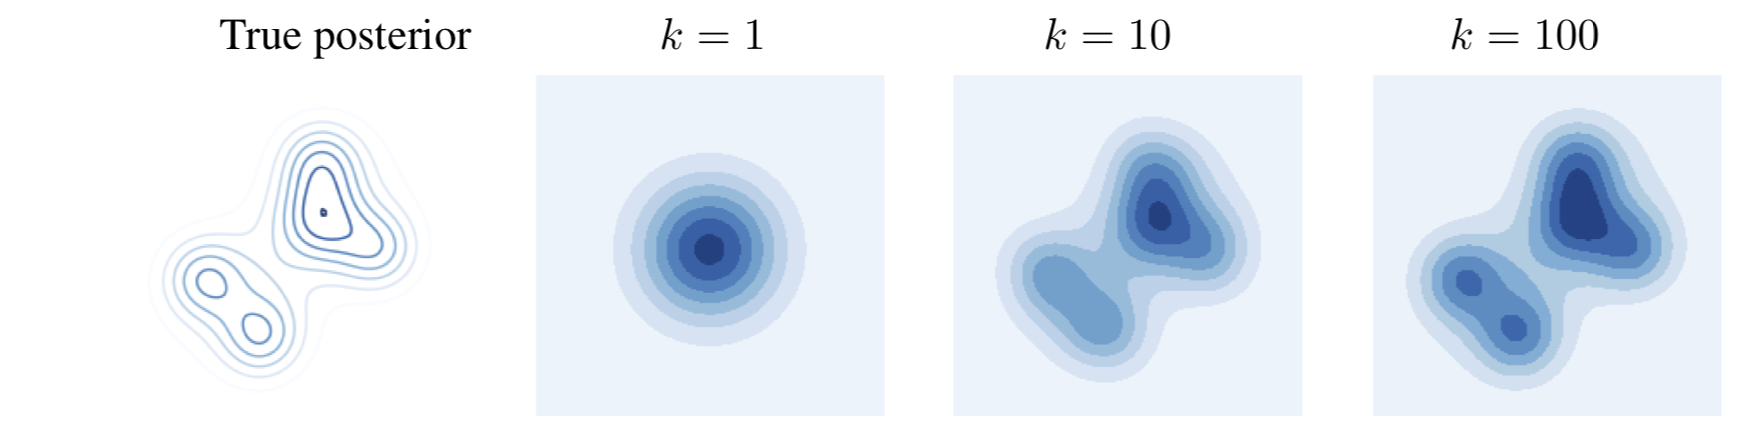
\includegraphics[width=\linewidth]{figs/IWAE_1.png}
\end{figure}
\begin{figure}
	\centering
	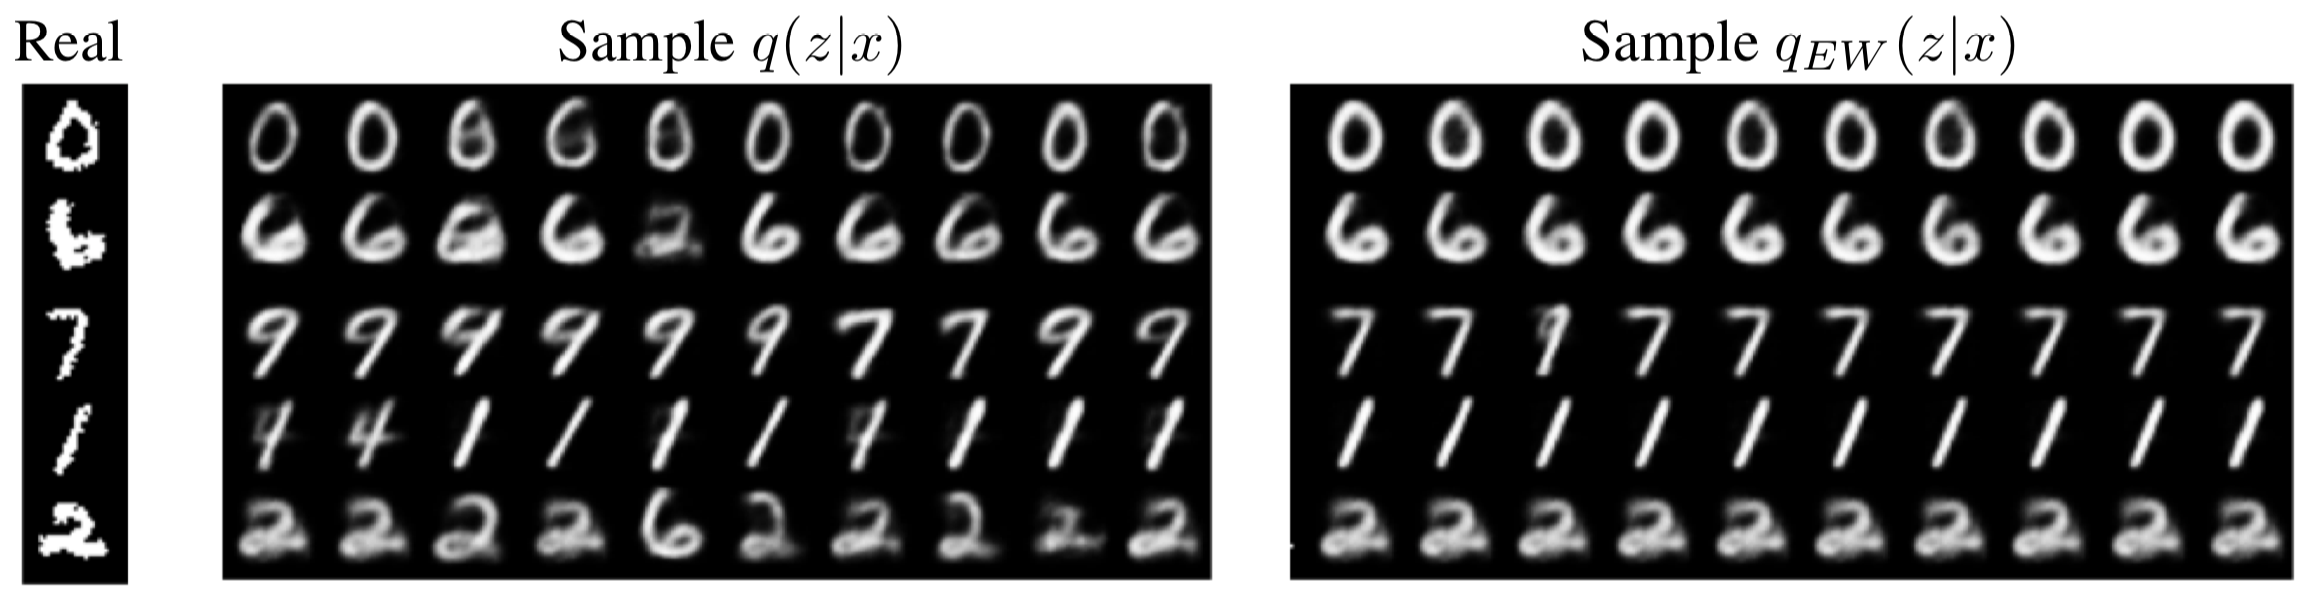
\includegraphics[width=\linewidth]{figs/IWAE_2.png}
\end{figure}

\vfill
\hrule\medskip
{\scriptsize \href{https://openreview.net/pdf?id=Syw2ZgrFx}{https://openreview.net/pdf?id=Syw2ZgrFx}}
\end{frame}
%=======
\begin{frame}{Summary}
	\begin{itemize}
		\item ELBO surgery reveals insights about prior distribution in VAE. The optimal prior is aggregated posterior.
		\item VampPrior proposed to use variational mixture of posteriors as prior to approximate the aggregated posterior.
		\item More powerful decoder in VAE leads to more expressive generative model. However, too expressive decoder could lead to posterior collapse.
		\item Decoder weakening is a set of techniques to avoid posterior collapse.
		\item Autoregressive flows could be used in prior. This is equivalent to the use of IAF posterior. 
		\item Importance sampling could get tighter lower bound to the likelihood.
	\end{itemize}
\end{frame}
%=======
\begin{frame}{References}
{\tiny
\begin{itemize}
	
	\item VAE with a \textbf{VampPrior} \\
	\href{https://arxiv.org/pdf/1705.07120.pdf}{https://arxiv.org/pdf/1705.07120.pdf} \\
	\textbf{Summary:} Variational Mixture of Posteriors prior is introduced. The VampPrior components are given by variational \\ posteriors conditioned on learnable pseudo-inputs. Prior is extended to a two layer hierarchical model with a coupled prior \\ and posterior, it learns significantly better models. The model avoids the local optima issues related to useless latent \\ dimensions that plague VAEs. The prior is compared with standard gaussian and mixture of gaussians.
	
    \item \textbf{PixelVAE:} A Latent Variable Model for Natural Images \\
    \href{https://arxiv.org/pdf/1611.05013.pdf}{https://arxiv.org/pdf/1611.05013.pdf} \\
    \textbf{Summary:} Use autoregressive model (PixelCNN) in VAE decoder. Use hierarchical structure of latent variables. Restrict the number of conv layers in PixelCNN (receptive field) to encode global structure in latent space. The performance is slightly worse than GatedPixelCNN.
    
    \item Improving Variational Inference with Inverse Autoregressive Flow \\
    \href{https://arxiv.org/abs/1606.04934}{https://arxiv.org/abs/1606.04934} \\
    \textbf{Summary:} Free bits proposed to weaken autoregressive decoder.
    
    \item \textbf{VLAE:} Variational Lossy Autoencoder \\
    \href{https://arxiv.org/abs/1611.02731}{https://arxiv.org/abs/1611.02731} \\
    \textbf{Summary:} Bits-back coding interpretation for posterior collapse. Solving the problem of ignoring latent codes. Reduce \\ receptive field in PixelCNN decoder to encode global information, use learnable AF prior.
    
    \item \textbf{IWAE}: Importance Weighted Autoencoders \\
    \href{https://arxiv.org/pdf/1509.00519.pdf}{https://arxiv.org/pdf/1509.00519.pdf} \\
    \textbf{Summary:} Propose the version of ELBO which is tighter to the log-density. Sampling of k objects from latent space instead of one. The more samples we samples the more tight the gap is. In the limit we will get the true likelihood. The gradient is given by importance sampling reweighting. Analyze the number of active latent units.
    
    \item Reinterpreting Importance-Weighted Autoencoders \\
    \href{https://arxiv.org/abs/1704.02916}{https://arxiv.org/abs/1704.02916} \\
    \textbf{Summary:} IWAE maximizes a tighter ELBO than VAE ELBO. This ELBO is also related to some implicit variational distribution. The analytical form of this distribution is given and visualized. 
    
\end{itemize}
}
\end{frame}
%=======
\begin{frame}{IWAE}
\[
\frac{a_1 + \dots + a_K}{K} = \mathbb{E}_{i_1, \dots, i_M} \frac{a_{i_1} + \dots + a_{i_M}}{M}, \quad i_1, \dots, i_M \sim U[1, K]
\]
\end{frame}

\end{document} 